\documentclass[a4paper]{article}
\usepackage[utf8]{inputenc}
\usepackage{amsmath}
\usepackage[colorinlistoftodos]{todonotes}
\usepackage[utf8]{inputenc}
\usepackage{graphicx}
\graphicspath{ {figures/} }
\usepackage{array}
\usepackage{placeins}
\usepackage[left=0.5 in,top=0.5in,right=0.5 in,bottom=0.5in]{geometry}
\PassOptionsToPackage{hyphens}{url}
\usepackage{hyperref}
\usepackage{parskip}
\usepackage [english]{babel}
\usepackage [autostyle, english = american]{csquotes}
\MakeOuterQuote{"}
\hypersetup{
     colorlinks,
     urlcolor    = blue
}
\usepackage{xcolor}
\usepackage{listings}
\lstloadlanguages{Python}
\newcommand{\inlinecode}[1]{\lstinline{#1}}

\lstset{
  language=Python,
  basicstyle=\scriptsize\sffamily,
  numberstyle=\color{gray},
  stringstyle=\color[HTML]{933797},
  commentstyle=\color[HTML]{228B22}\sffamily,
  emph={[2]from,import,pass,return}, emphstyle={[2]\color[HTML]{DD52F0}},
  emph={[3]range}, emphstyle={[3]\color[HTML]{D17032}},
  emph={[4]for,in,def}, emphstyle={[4]\color{blue}},
  showstringspaces=false,
  breaklines=true,
  prebreak=\mbox{{\color{gray}\tiny$\searrow$}},
  numbers=left,
  xleftmargin=15pt
}

\title{Application 3: Closest Pairs and Clustering \\Algorithmic Thinking (Part2)}
\author{Shamsuddin Rehmani}
\begin{document}
\sloppy
\maketitle
\section*{Application 3 Description}
In Project 3, you implemented two methods for clustering sets of data. In this Application, we will analyze the performance of these two methods on various subsets of our county-level cancer risk data set. In particular, we will compare these two clustering methods in three areas:

\begin{itemize}
	\item Efficiency - Which method computes clusterings more efficiently?
	\item Automation - Which method requires less human supervision to generate reasonable clusterings?
	\item Quality - Which method generates clusterings with less error?
\end{itemize}


\section*{Answer to Question 1}
\FloatBarrier
% trim=l b r t
\begin{figure}[h]
	\centering 
	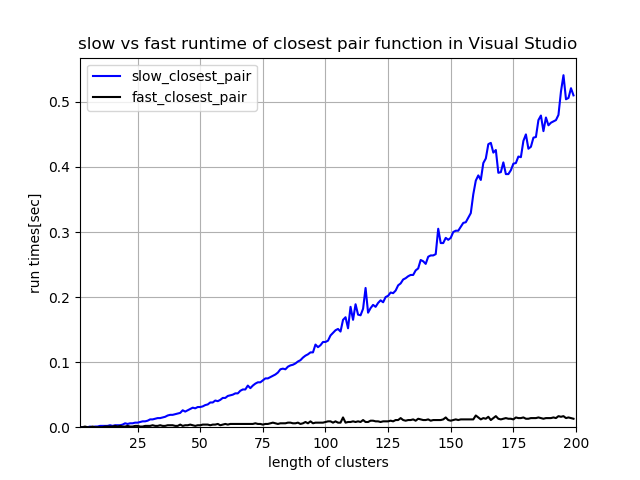
\includegraphics[scale = 1.0, clip=false, trim=0cm 0cm 0cm 0cm]{Q1_closest_pair_comparision.png}
	\caption{Fast vs slow closest pair function runtime comparison}
\end{figure}
\FloatBarrier

\newpage
\section*{Answer to Question 2}

\FloatBarrier
% trim=l b r t
\begin{figure}[h]
	\centering 
	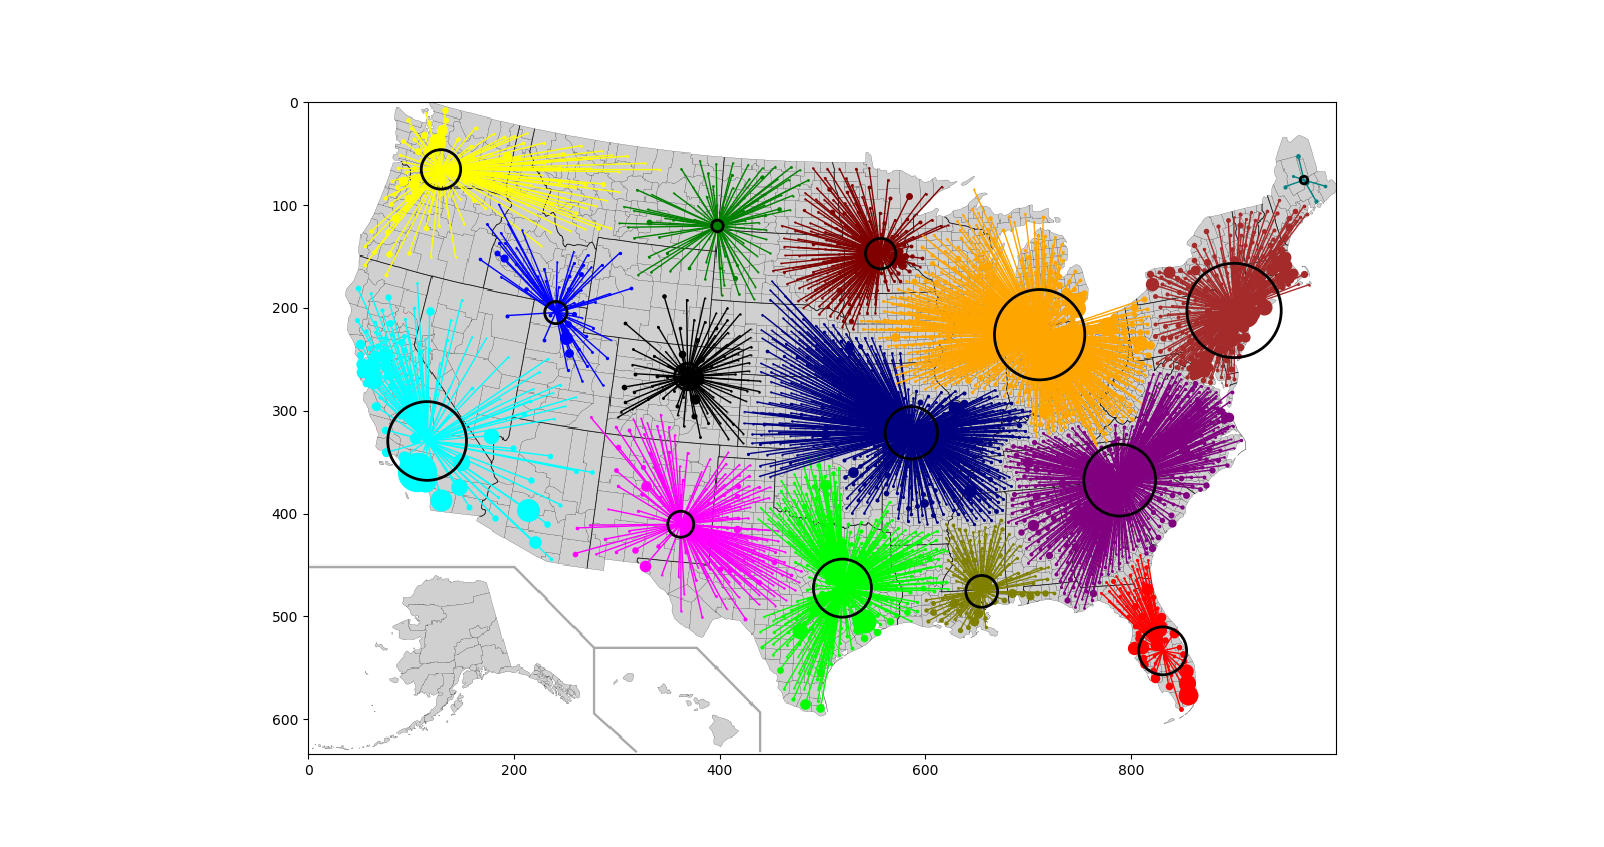
\includegraphics[scale = 0.5, clip=True, trim=5.5cm 1.5cm 0cm 2.5cm]{Q2_hierarchical.png}
	\caption{15 clusters generated by hierarchical clustering for 3108 counties}
\end{figure}
\FloatBarrier


\section*{Answer to Question 3}

\FloatBarrier
% trim=l b r t
\begin{figure}[h]
	\centering 
	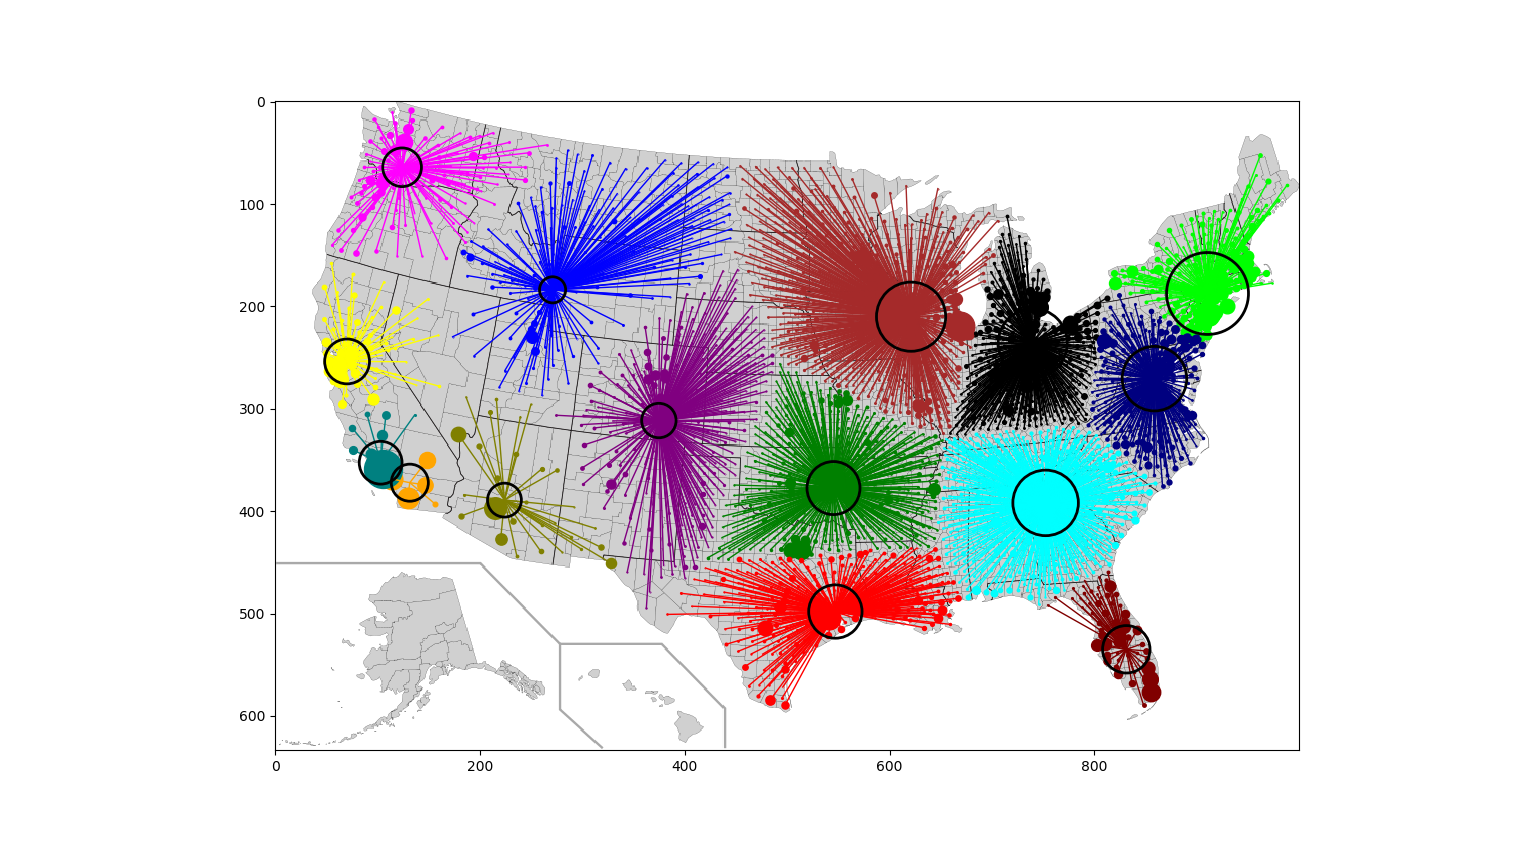
\includegraphics[scale = 0.5, clip=True, trim=5.5cm 1.5cm 0cm 2.5cm]{Q3_clustering_k_mean.png}
	\caption{15 clusters with 5 iterations generated by k-mean clustering for 3108 counties}
\end{figure}
\FloatBarrier

\section*{Answer to Question 4}

let $k =$ number of clusters

$n = $ size of the input cluster list

$q = $ number of iterations (for k-mean clustering)

Then for hierarchical clustering, the time complexity is $O((n - k)(nlog(n) + n{log(n)}^2))$
which is $~ O(n^2(logn)^2)$ if $k$ is small compared to $n$ as stated in the above question

On the other hand, the time complexity of k-mean clustering is $~ O(qnk)$. Since $k$ is small
compared to $n$ and $q$ is also a small fixed number, time complexity is $O(n)$ which is much more
efficient than heirarchiacl clustering 


\section*{Answer to Question 5}
\FloatBarrier
% trim=l b r t
\begin{figure}[h]
	\centering 
	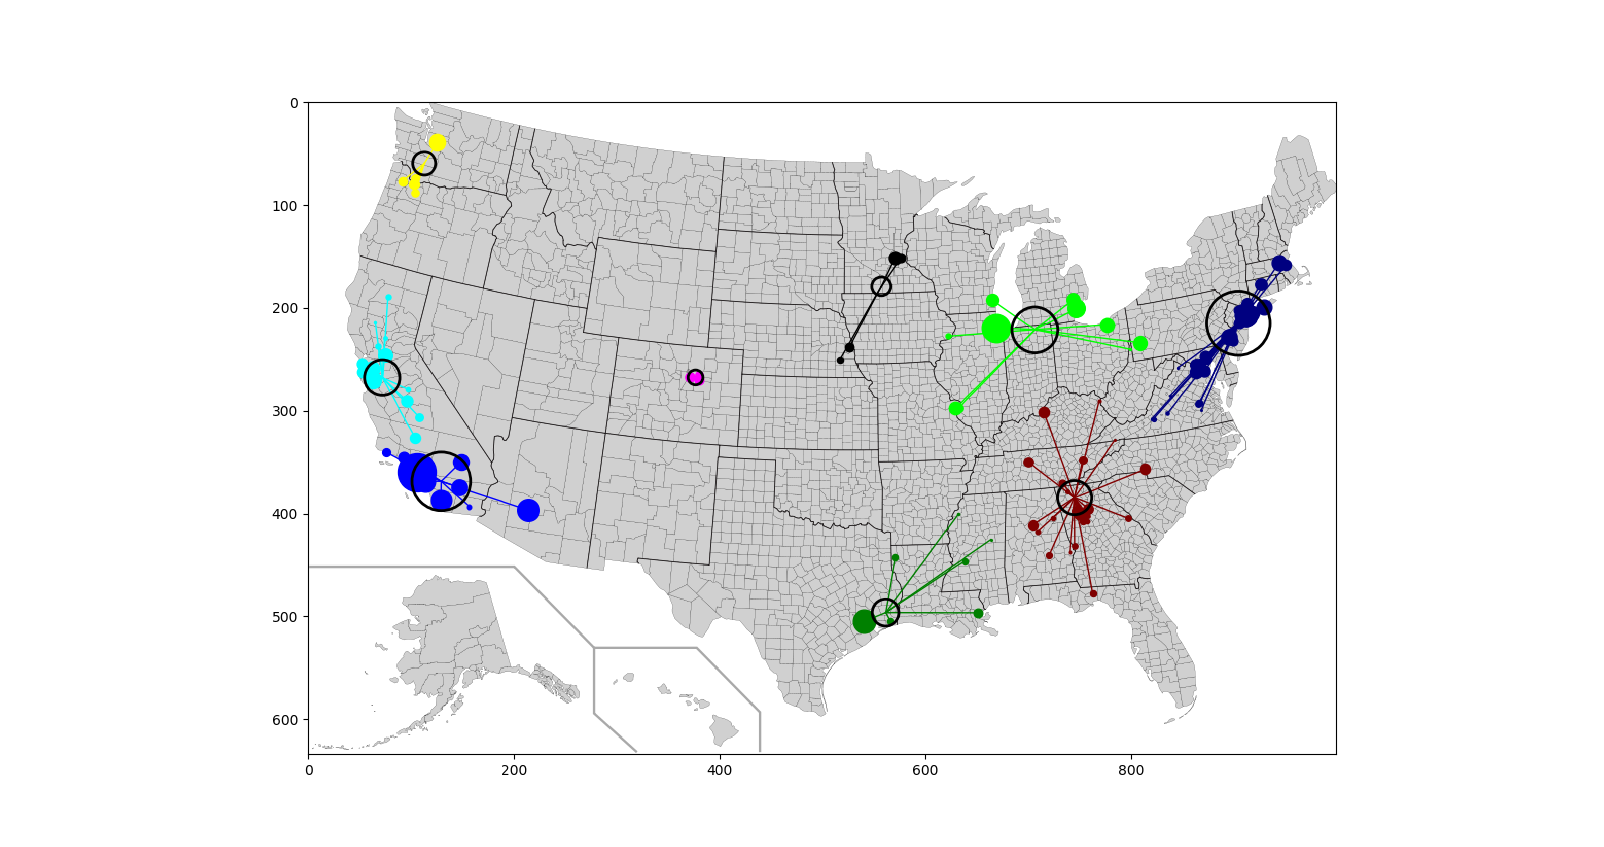
\includegraphics[scale = 0.5, clip=True, trim=5.5cm 1.5cm 0cm 2.5cm]{Q5_hierarchical.png}
		\caption{9 clusters generated by hierarchical clustering for 111 counties}
\end{figure}
\FloatBarrier

\section*{Answer to Question 6}
\FloatBarrier
% trim=l b r t
\begin{figure}[h]
	\centering 
	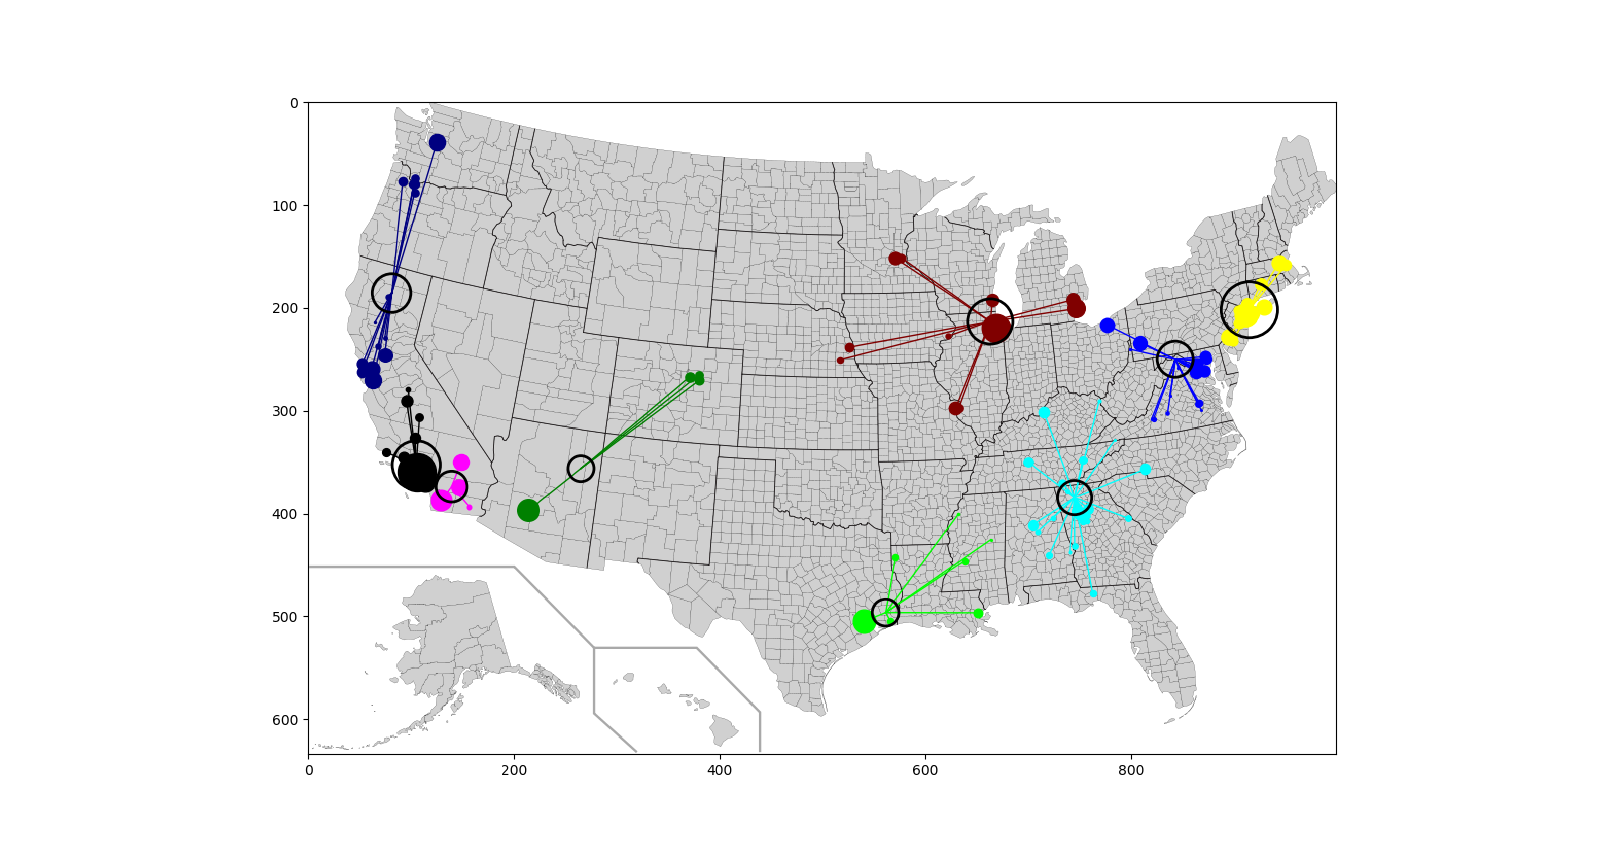
\includegraphics[scale = 0.5, clip=True, trim=5.5cm 1.5cm 0cm 2.5cm]{Q6_clustering_k_mean.png}
	\caption{9 clusters with 5 iterations generated by k-mean clustering for 111 counties}
\end{figure}
\FloatBarrier
 

\section*{Answer to Question 7}

Distortion of hierarchical clustering for 111 counties: $1.75 \times 10^{11}$ 

Distortion of k-mean clustering for 111 counties: $2.71 \times 10^{11}$

\section*{Answer to Question 8}
For the k-mean clustering(Figure 5) we can see that the 3 cluster centers are located in the california region (one in northern while two in southern region) while of the 3 centers for the hierarchical clustering one is located in Washington state  and two in the california region. The high distortion for the k-mean is due to the fact that the counties in the cluster with center in the northern California is distrbuted in Washington and southern California i.e the counties are much further than the center. The difference between the distortion values is becauses the intial clustering method for k-mean involves clustering around counties with highest population. Due to this all 3 counties(3 largest circles are black and pink) in the southern California were included in the intial clustering while none from Washington, Oregon or Northern California was selected. Thus this resulted in relatively higher distortion.

\section*{Answer to Question 9}
Based on Question 8, we say that hierarchical clustering requires less human supervision as it requires only choosing the number of ouput clusters. While on the other hand, for k-mean we need a good choice of the intial cluster centers.

\section*{Answer to Question 10}
\FloatBarrier
% trim=l b r t
\begin{figure}[h]
	\centering 
	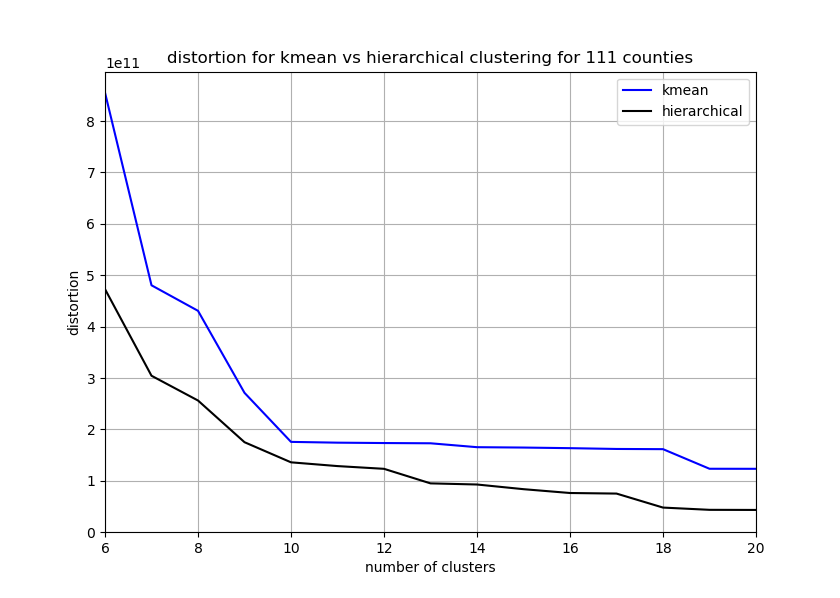
\includegraphics[scale = 0.8, clip=True, trim=1cm 1cm 0cm 1cm]{Q10_distortion_111.png}
	\caption{9 clusters with 5 iterations generated by k-mean clustering for 111 counties}
\end{figure}
\FloatBarrier

\FloatBarrier
% trim=l b r t
\begin{figure}[h]
	\centering 
	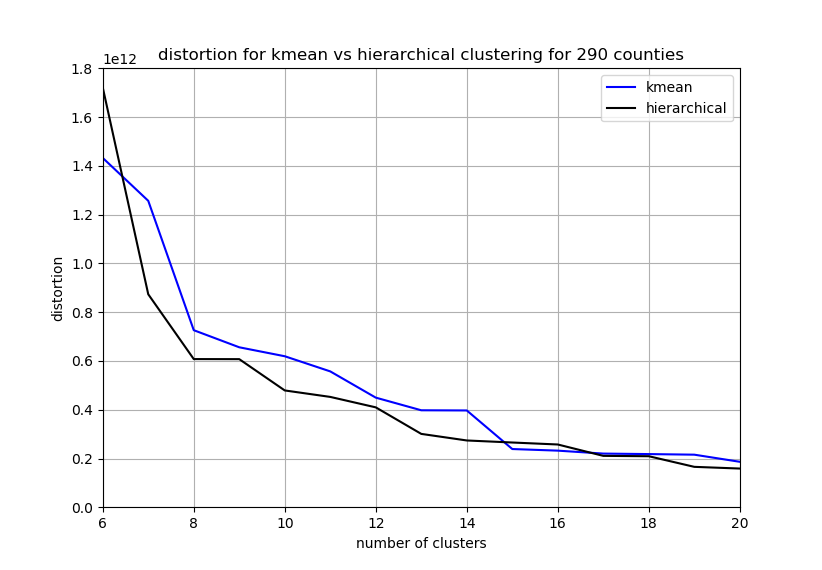
\includegraphics[scale = 0.8, clip=True, trim=1cm 1cm 0cm 1cm]{Q10_distortion_290.png}
	\caption{9 clusters with 5 iterations generated by k-mean clustering for 111 counties}
\end{figure}
\FloatBarrier

\FloatBarrier
% trim=l b r t
\begin{figure}[h]
	\centering 
	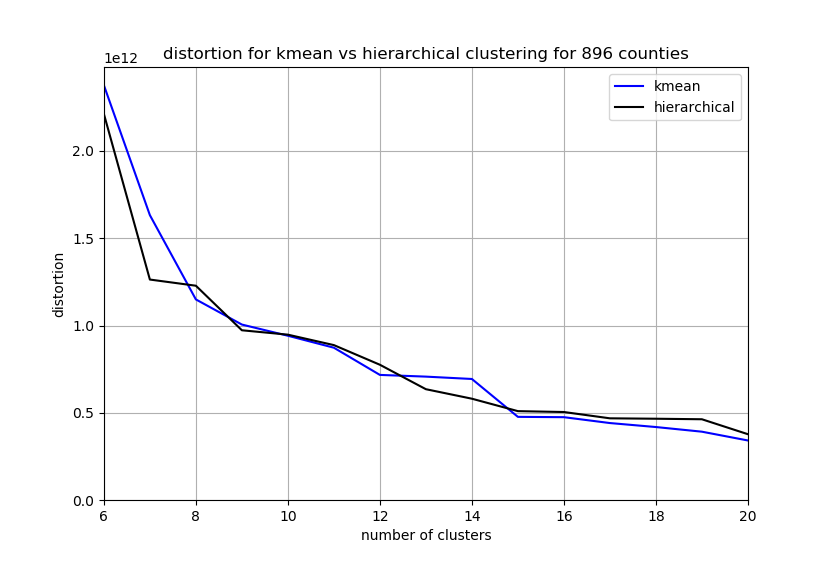
\includegraphics[scale = 0.8, clip=True, trim=1cm 1cm 0cm 1cm]{Q10_distortion_896.png}
	\caption{9 clusters with 5 iterations generated by k-mean clustering for 111 counties}
\end{figure}
\FloatBarrier

\newpage
\appendix
\section{Python code used to answer the Application Questions}
\lstinputlisting{alg_application3_solution.py}
\section{All functions for project 4 used in the application}
\lstinputlisting{alg_project3_solution.py}

\end{document}
